% Figure 2: Lean4 Module Dependency Graph
% For inclusion in main.tex via % Figure 2: Lean4 Module Dependency Graph
%
% This file contains TikZ code for the module dependency diagram.
% Can be compiled standalone or included in main.tex
%
% SPECIFICATION:
% - Show all 8 Lean4 modules as nodes
% - Directed edges showing import dependencies
% - Module statistics (theorems count) as labels
% - Layered layout: foundational at top, derived at bottom
% - Color coding by category

\documentclass[tikz,border=10pt]{standalone}
\usepackage{tikz}
\usetikzlibrary{arrows.meta,shapes,positioning,calc}

\begin{document}
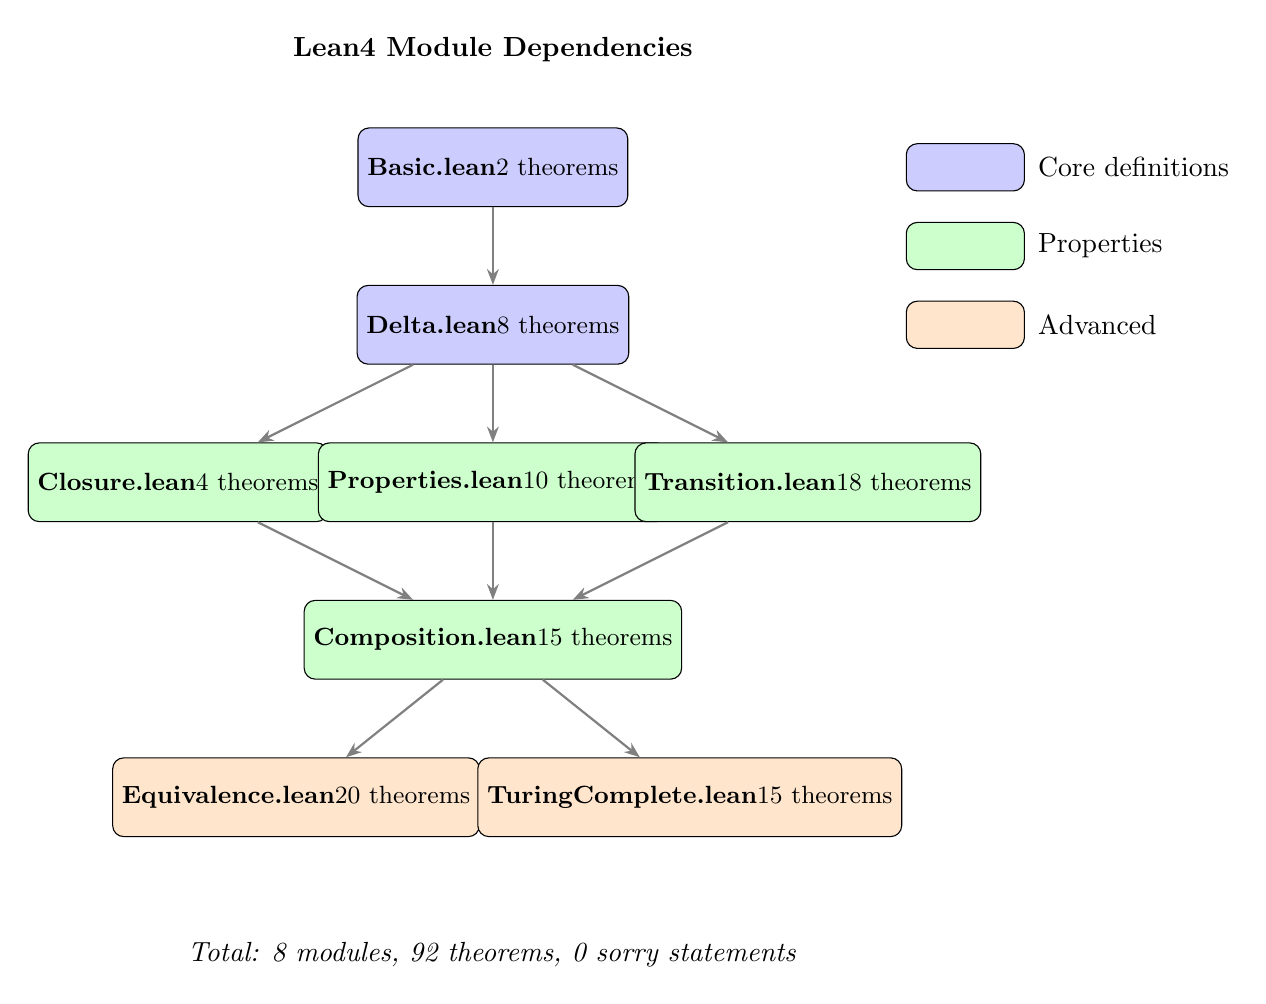
\begin{tikzpicture}[
    module/.style={draw, rectangle, rounded corners, minimum width=3cm, minimum height=1cm, font=\small},
    core/.style={module, fill=blue!20},
    props/.style={module, fill=green!20},
    advanced/.style={module, fill=orange!20},
    arrow/.style={-{Stealth[length=2mm]}, thick, gray}
]

% Layer 1: Foundation
\node[core] (basic) at (0, 0) {\textbf{Basic.lean}\\2 theorems};

% Layer 2: Core types
\node[core] (delta) at (0, -2) {\textbf{Delta.lean}\\8 theorems};

% Layer 3: Properties (parallel)
\node[props] (closure) at (-4, -4) {\textbf{Closure.lean}\\4 theorems};
\node[props] (props) at (0, -4) {\textbf{Properties.lean}\\10 theorems};
\node[props] (trans) at (4, -4) {\textbf{Transition.lean}\\18 theorems};

% Layer 4: Composition
\node[props] (comp) at (0, -6) {\textbf{Composition.lean}\\15 theorems};

% Layer 5: Advanced (parallel)
\node[advanced] (equiv) at (-2.5, -8) {\textbf{Equivalence.lean}\\20 theorems};
\node[advanced] (turing) at (2.5, -8) {\textbf{TuringComplete.lean}\\15 theorems};

% Arrows
\draw[arrow] (basic) -- (delta);
\draw[arrow] (delta) -- (closure);
\draw[arrow] (delta) -- (props);
\draw[arrow] (delta) -- (trans);
\draw[arrow] (closure) -- (comp);
\draw[arrow] (props) -- (comp);
\draw[arrow] (trans) -- (comp);
\draw[arrow] (comp) -- (equiv);
\draw[arrow] (comp) -- (turing);

% Legend
\node[core, minimum width=1.5cm, minimum height=0.6cm] at (6, 0) {};
\node[right] at (6.8, 0) {Core definitions};
\node[props, minimum width=1.5cm, minimum height=0.6cm] at (6, -1) {};
\node[right] at (6.8, -1) {Properties};
\node[advanced, minimum width=1.5cm, minimum height=0.6cm] at (6, -2) {};
\node[right] at (6.8, -2) {Advanced};

% Title
\node at (0, 1.5) {\textbf{Lean4 Module Dependencies}};

% Total
\node at (0, -10) {\textit{Total: 8 modules, 92 theorems, 0 sorry statements}};

\end{tikzpicture}
\end{document}


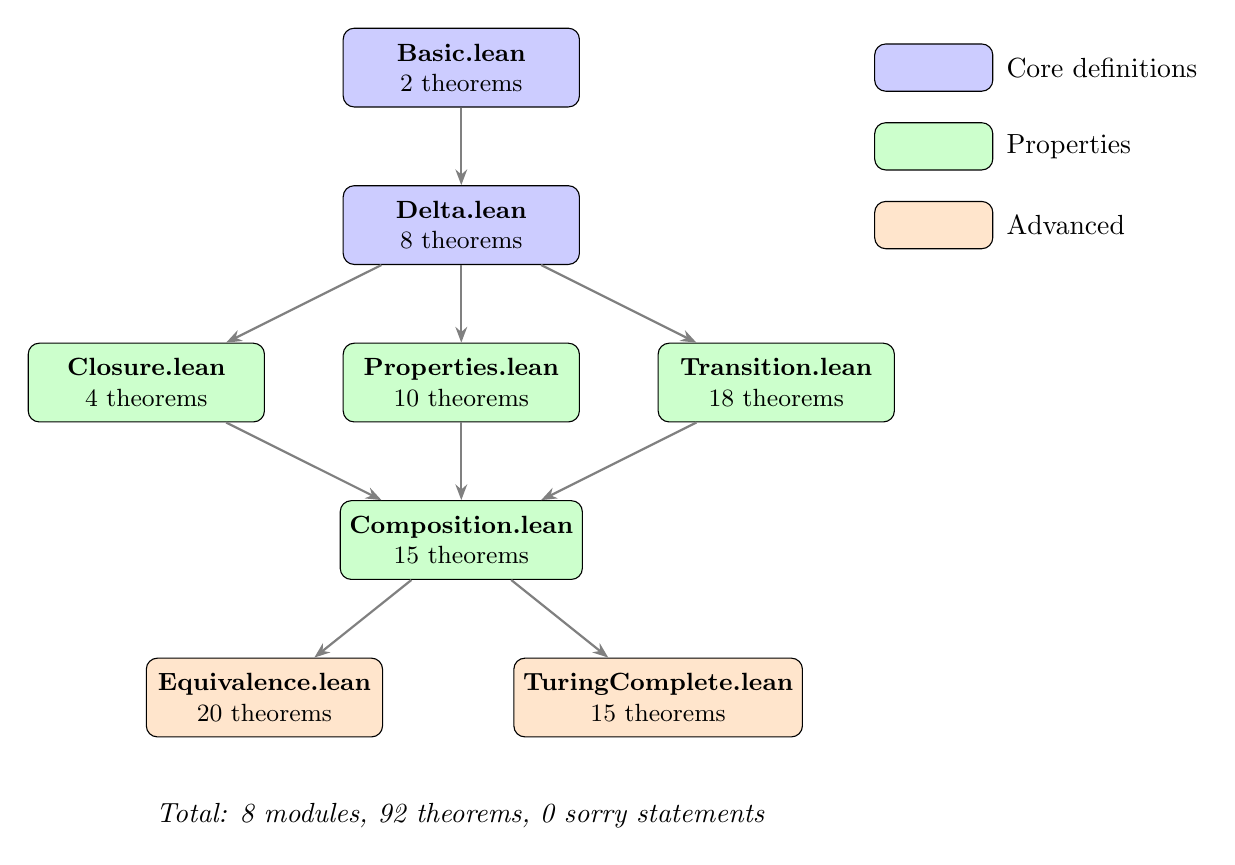
\begin{tikzpicture}[
    module/.style={draw, rectangle, rounded corners, minimum width=3cm, minimum height=1cm, font=\small, align=center},
    core/.style={module, fill=blue!20},
    props/.style={module, fill=green!20},
    advanced/.style={module, fill=orange!20},
    arrow/.style={-{Stealth[length=2mm]}, thick, gray}
]

% Layer 1: Foundation
\node[core] (basic) at (0, 0) {\textbf{Basic.lean}\\2 theorems};

% Layer 2: Core types
\node[core] (delta) at (0, -2) {\textbf{Delta.lean}\\8 theorems};

% Layer 3: Properties (parallel)
\node[props] (closure) at (-4, -4) {\textbf{Closure.lean}\\4 theorems};
\node[props] (props) at (0, -4) {\textbf{Properties.lean}\\10 theorems};
\node[props] (trans) at (4, -4) {\textbf{Transition.lean}\\18 theorems};

% Layer 4: Composition
\node[props] (comp) at (0, -6) {\textbf{Composition.lean}\\15 theorems};

% Layer 5: Advanced (parallel)
\node[advanced] (equiv) at (-2.5, -8) {\textbf{Equivalence.lean}\\20 theorems};
\node[advanced] (turing) at (2.5, -8) {\textbf{TuringComplete.lean}\\15 theorems};

% Arrows
\draw[arrow] (basic) -- (delta);
\draw[arrow] (delta) -- (closure);
\draw[arrow] (delta) -- (props);
\draw[arrow] (delta) -- (trans);
\draw[arrow] (closure) -- (comp);
\draw[arrow] (props) -- (comp);
\draw[arrow] (trans) -- (comp);
\draw[arrow] (comp) -- (equiv);
\draw[arrow] (comp) -- (turing);

% Legend
\node[core, minimum width=1.5cm, minimum height=0.6cm] at (6, 0) {};
\node[right] at (6.8, 0) {Core definitions};
\node[props, minimum width=1.5cm, minimum height=0.6cm] at (6, -1) {};
\node[right] at (6.8, -1) {Properties};
\node[advanced, minimum width=1.5cm, minimum height=0.6cm] at (6, -2) {};
\node[right] at (6.8, -2) {Advanced};

% Total
\node at (0, -9.5) {\textit{Total: 8 modules, 92 theorems, 0 sorry statements}};

\end{tikzpicture}
